\documentclass[1p]{elsarticle_modified}
%\bibliographystyle{elsarticle-num}

%\usepackage[colorlinks]{hyperref}
%\usepackage{abbrmath_seonhwa} %\Abb, \Ascr, \Acal ,\Abf, \Afrak
\usepackage{amsfonts}
\usepackage{amssymb}
\usepackage{amsmath}
\usepackage{amsthm}
\usepackage{scalefnt}
\usepackage{amsbsy}
\usepackage{kotex}
\usepackage{caption}
\usepackage{subfig}
\usepackage{color}
\usepackage{graphicx}
\usepackage{xcolor} %% white, black, red, green, blue, cyan, magenta, yellow
\usepackage{float}
\usepackage{setspace}
\usepackage{hyperref}

\usepackage{tikz}
\usetikzlibrary{arrows}

\usepackage{multirow}
\usepackage{array} % fixed length table
\usepackage{hhline}

%%%%%%%%%%%%%%%%%%%%%
\makeatletter
\renewcommand*\env@matrix[1][\arraystretch]{%
	\edef\arraystretch{#1}%
	\hskip -\arraycolsep
	\let\@ifnextchar\new@ifnextchar
	\array{*\c@MaxMatrixCols c}}
\makeatother %https://tex.stackexchange.com/questions/14071/how-can-i-increase-the-line-spacing-in-a-matrix
%%%%%%%%%%%%%%%

\usepackage[normalem]{ulem}

\newcommand{\msout}[1]{\ifmmode\text{\sout{\ensuremath{#1}}}\else\sout{#1}\fi}
%SOURCE: \msout is \stkout macro in https://tex.stackexchange.com/questions/20609/strikeout-in-math-mode

\newcommand{\cancel}[1]{
	\ifmmode
	{\color{red}\msout{#1}}
	\else
	{\color{red}\sout{#1}}
	\fi
}

\newcommand{\add}[1]{
	{\color{blue}\uwave{#1}}
}

\newcommand{\replace}[2]{
	\ifmmode
	{\color{red}\msout{#1}}{\color{blue}\uwave{#2}}
	\else
	{\color{red}\sout{#1}}{\color{blue}\uwave{#2}}
	\fi
}

\newcommand{\Sol}{\mathcal{S}} %segment
\newcommand{\D}{D} %diagram
\newcommand{\A}{\mathcal{A}} %arc


%%%%%%%%%%%%%%%%%%%%%%%%%%%%%5 test

\def\sl{\operatorname{\textup{SL}}(2,\Cbb)}
\def\psl{\operatorname{\textup{PSL}}(2,\Cbb)}
\def\quan{\mkern 1mu \triangleright \mkern 1mu}

\theoremstyle{definition}
\newtheorem{thm}{Theorem}[section]
\newtheorem{prop}[thm]{Proposition}
\newtheorem{lem}[thm]{Lemma}
\newtheorem{ques}[thm]{Question}
\newtheorem{cor}[thm]{Corollary}
\newtheorem{defn}[thm]{Definition}
\newtheorem{exam}[thm]{Example}
\newtheorem{rmk}[thm]{Remark}
\newtheorem{alg}[thm]{Algorithm}

\newcommand{\I}{\sqrt{-1}}
\begin{document}

%\begin{frontmatter}
%
%\title{Boundary parabolic representations of knots up to 8 crossings}
%
%%% Group authors per affiliation:
%\author{Yunhi Cho} 
%\address{Department of Mathematics, University of Seoul, Seoul, Korea}
%\ead{yhcho@uos.ac.kr}
%
%
%\author{Seonhwa Kim} %\fnref{s_kim}}
%\address{Center for Geometry and Physics, Institute for Basic Science, Pohang, 37673, Korea}
%\ead{ryeona17@ibs.re.kr}
%
%\author{Hyuk Kim}
%\address{Department of Mathematical Sciences, Seoul National University, Seoul 08826, Korea}
%\ead{hyukkim@snu.ac.kr}
%
%\author{Seokbeom Yoon}
%\address{Department of Mathematical Sciences, Seoul National University, Seoul, 08826,  Korea}
%\ead{sbyoon15@snu.ac.kr}
%
%\begin{abstract}
%We find all boundary parabolic representation of knots up to 8 crossings.
%
%\end{abstract}
%\begin{keyword}
%    \MSC[2010] 57M25 
%\end{keyword}
%
%\end{frontmatter}

%\linenumbers
%\tableofcontents
%
\newcommand\colored[1]{\textcolor{white}{\rule[-0.35ex]{0.8em}{1.4ex}}\kern-0.8em\color{red} #1}%
%\newcommand\colored[1]{\textcolor{white}{ #1}\kern-2.17ex	\textcolor{white}{ #1}\kern-1.81ex	\textcolor{white}{ #1}\kern-2.15ex\color{red}#1	}

{\Large $\underline{12a_{0633}~(K12a_{0633})}$}

\setlength{\tabcolsep}{10pt}
\renewcommand{\arraystretch}{1.6}
\vspace{1cm}\begin{tabular}{m{100pt}>{\centering\arraybackslash}m{274pt}}
\multirow{5}{120pt}{
	\centering
	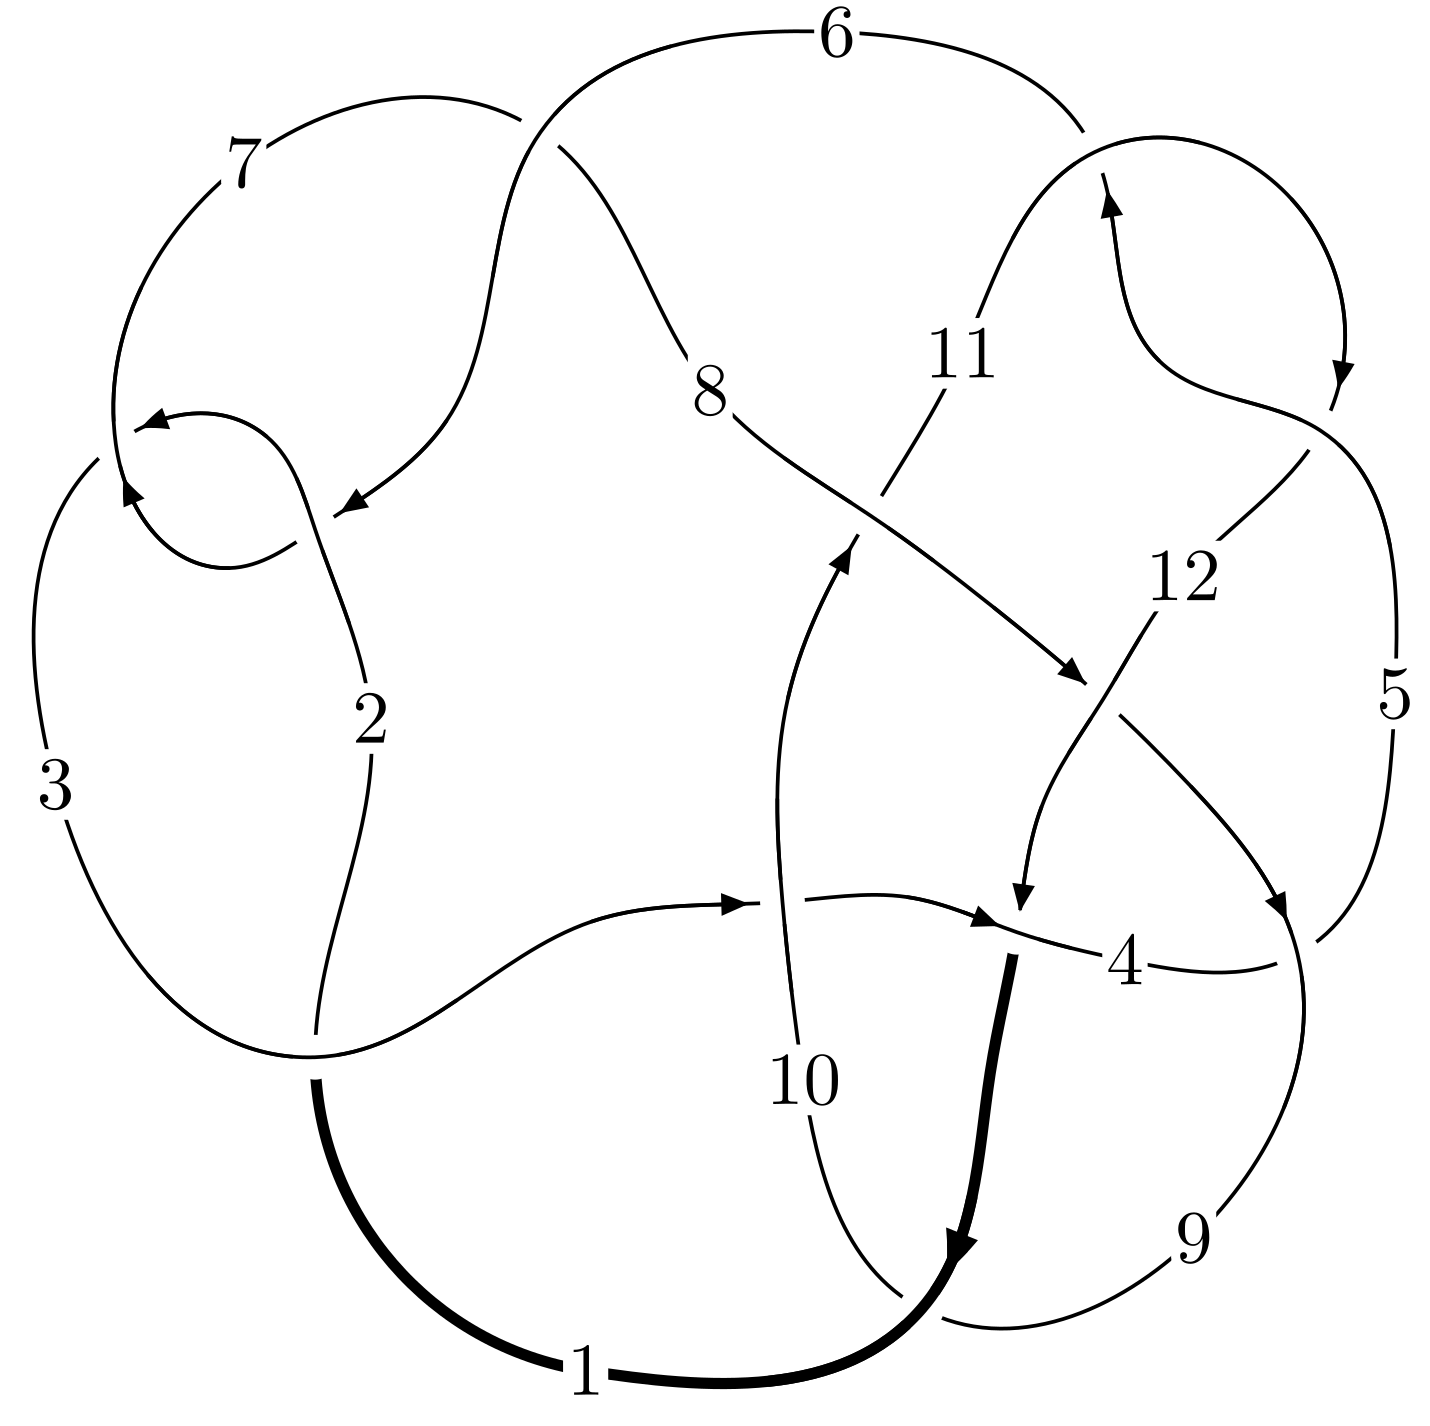
\includegraphics[width=112pt]{../../../GIT/diagram.site/Diagrams/png/1434_12a_0633.png}\\
\ \ \ A knot diagram\footnotemark}&
\allowdisplaybreaks
\textbf{Linearized knot diagam} \\
\cline{2-2}
 &
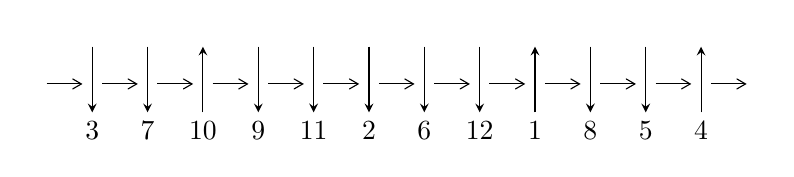
\begin{tikzpicture}[x=20pt, y=17pt]
	% nodes
	\node (C0) at (0, 0) {};
	\node (C1) at (1, 0) {};
	\node (C1U) at (1, +1) {};
	\node (C1D) at (1, -1) {3};

	\node (C2) at (2, 0) {};
	\node (C2U) at (2, +1) {};
	\node (C2D) at (2, -1) {7};

	\node (C3) at (3, 0) {};
	\node (C3U) at (3, +1) {};
	\node (C3D) at (3, -1) {10};

	\node (C4) at (4, 0) {};
	\node (C4U) at (4, +1) {};
	\node (C4D) at (4, -1) {9};

	\node (C5) at (5, 0) {};
	\node (C5U) at (5, +1) {};
	\node (C5D) at (5, -1) {11};

	\node (C6) at (6, 0) {};
	\node (C6U) at (6, +1) {};
	\node (C6D) at (6, -1) {2};

	\node (C7) at (7, 0) {};
	\node (C7U) at (7, +1) {};
	\node (C7D) at (7, -1) {6};

	\node (C8) at (8, 0) {};
	\node (C8U) at (8, +1) {};
	\node (C8D) at (8, -1) {12};

	\node (C9) at (9, 0) {};
	\node (C9U) at (9, +1) {};
	\node (C9D) at (9, -1) {1};

	\node (C10) at (10, 0) {};
	\node (C10U) at (10, +1) {};
	\node (C10D) at (10, -1) {8};

	\node (C11) at (11, 0) {};
	\node (C11U) at (11, +1) {};
	\node (C11D) at (11, -1) {5};

	\node (C12) at (12, 0) {};
	\node (C12U) at (12, +1) {};
	\node (C12D) at (12, -1) {4};
	\node (C13) at (13, 0) {};

	% arrows
	\draw[->,>={angle 60}]
	(C0) edge (C1) (C1) edge (C2) (C2) edge (C3) (C3) edge (C4) (C4) edge (C5) (C5) edge (C6) (C6) edge (C7) (C7) edge (C8) (C8) edge (C9) (C9) edge (C10) (C10) edge (C11) (C11) edge (C12) (C12) edge (C13) ;	\draw[->,>=stealth]
	(C1U) edge (C1D) (C2U) edge (C2D) (C3D) edge (C3U) (C4U) edge (C4D) (C5U) edge (C5D) (C6U) edge (C6D) (C7U) edge (C7D) (C8U) edge (C8D) (C9D) edge (C9U) (C10U) edge (C10D) (C11U) edge (C11D) (C12D) edge (C12U) ;
	\end{tikzpicture} \\
\hhline{~~} \\& 
\textbf{Solving Sequence} \\ \cline{2-2} 
 &
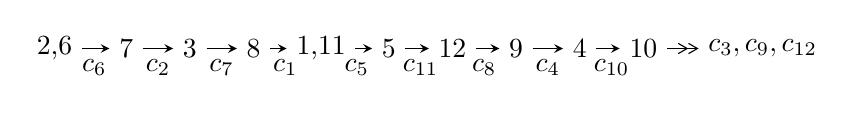
\begin{tikzpicture}[x=23pt, y=7pt]
	% node
	\node (A0) at (-1/8, 0) {2,6};
	\node (A1) at (1, 0) {7};
	\node (A2) at (2, 0) {3};
	\node (A3) at (3, 0) {8};
	\node (A4) at (65/16, 0) {1,11};
	\node (A5) at (41/8, 0) {5};
	\node (A6) at (49/8, 0) {12};
	\node (A7) at (57/8, 0) {9};
	\node (A8) at (65/8, 0) {4};
	\node (A9) at (73/8, 0) {10};
	\node (C1) at (1/2, -1) {$c_{6}$};
	\node (C2) at (3/2, -1) {$c_{2}$};
	\node (C3) at (5/2, -1) {$c_{7}$};
	\node (C4) at (7/2, -1) {$c_{1}$};
	\node (C5) at (37/8, -1) {$c_{5}$};
	\node (C6) at (45/8, -1) {$c_{11}$};
	\node (C7) at (53/8, -1) {$c_{8}$};
	\node (C8) at (61/8, -1) {$c_{4}$};
	\node (C9) at (69/8, -1) {$c_{10}$};
	\node (A10) at (11, 0) {$c_{3},c_{9},c_{12}$};

	% edge
	\draw[->,>=stealth]	
	(A0) edge (A1) (A1) edge (A2) (A2) edge (A3) (A3) edge (A4) (A4) edge (A5) (A5) edge (A6) (A6) edge (A7) (A7) edge (A8) (A8) edge (A9) ;
	\draw[->>,>={angle 60}]	
	(A9) edge (A10);
\end{tikzpicture} \\ 

\end{tabular} \\

\footnotetext{
The image of knot diagram is generated by the software ``\textbf{Draw programme}" developed by Andrew Bartholomew(\url{http://www.layer8.co.uk/maths/draw/index.htm\#Running-draw}), where we modified some parts for our purpose(\url{https://github.com/CATsTAILs/LinksPainter}).
}\phantom \\ \newline 
\centering \textbf{Ideals for irreducible components\footnotemark of $X_{\text{par}}$} 
 
\begin{align*}
I^u_{1}&=\langle 
-5.15499\times10^{196} u^{129}+3.24861\times10^{196} u^{128}+\cdots+1.37901\times10^{195} b-1.57265\times10^{198},\\
\phantom{I^u_{1}}&\phantom{= \langle  }-1.02606\times10^{197} u^{129}+6.86879\times10^{196} u^{128}+\cdots+1.37901\times10^{195} a-2.82868\times10^{198},\\
\phantom{I^u_{1}}&\phantom{= \langle  }u^{130}-18 u^{128}+\cdots+24 u+19\rangle \\
I^u_{2}&=\langle 
-13 u^{20}-15 u^{19}+\cdots+b+14,\;19 u^{20}+35 u^{19}+\cdots+a-59,\;u^{21}+u^{20}+\cdots- u+1\rangle \\
\\
\end{align*}
\raggedright * 2 irreducible components of $\dim_{\mathbb{C}}=0$, with total 151 representations.\\
\footnotetext{All coefficients of polynomials are rational numbers. But the coefficients are sometimes approximated in decimal forms when there is not enough margin.}
\newpage
\renewcommand{\arraystretch}{1}
\centering \section*{I. $I^u_{1}= \langle -5.15\times10^{196} u^{129}+3.25\times10^{196} u^{128}+\cdots+1.38\times10^{195} b-1.57\times10^{198},\;-1.03\times10^{197} u^{129}+6.87\times10^{196} u^{128}+\cdots+1.38\times10^{195} a-2.83\times10^{198},\;u^{130}-18 u^{128}+\cdots+24 u+19 \rangle$}
\flushleft \textbf{(i) Arc colorings}\\
\begin{tabular}{m{7pt} m{180pt} m{7pt} m{180pt} }
\flushright $a_{2}=$&$\begin{pmatrix}0\\u\end{pmatrix}$ \\
\flushright $a_{6}=$&$\begin{pmatrix}1\\0\end{pmatrix}$ \\
\flushright $a_{7}=$&$\begin{pmatrix}1\\u^2\end{pmatrix}$ \\
\flushright $a_{3}=$&$\begin{pmatrix}- u\\- u^3+u\end{pmatrix}$ \\
\flushright $a_{8}=$&$\begin{pmatrix}- u^2+1\\u^2\end{pmatrix}$ \\
\flushright $a_{1}=$&$\begin{pmatrix}u^3\\u^5- u^3+u\end{pmatrix}$ \\
\flushright $a_{11}=$&$\begin{pmatrix}74.4057 u^{129}-49.8096 u^{128}+\cdots-355.205 u+2051.24\\37.3818 u^{129}-23.5575 u^{128}+\cdots-376.747 u+1140.42\end{pmatrix}$ \\
\flushright $a_{5}=$&$\begin{pmatrix}139.212 u^{129}-96.6569 u^{128}+\cdots-847.639 u+3887.02\\141.255 u^{129}-98.2425 u^{128}+\cdots-673.486 u+3861.62\end{pmatrix}$ \\
\flushright $a_{12}=$&$\begin{pmatrix}604.791 u^{129}-416.864 u^{128}+\cdots-3262.60 u+16766.7\\548.815 u^{129}-376.029 u^{128}+\cdots-2908.26 u+15158.3\end{pmatrix}$ \\
\flushright $a_{9}=$&$\begin{pmatrix}75.2273 u^{129}-49.1018 u^{128}+\cdots-463.385 u+2139.10\\44.2171 u^{129}-27.8912 u^{128}+\cdots-437.538 u+1348.93\end{pmatrix}$ \\
\flushright $a_{4}=$&$\begin{pmatrix}174.835 u^{129}-119.982 u^{128}+\cdots-1033.66 u+4885.75\\147.231 u^{129}-101.881 u^{128}+\cdots-772.157 u+4071.79\end{pmatrix}$ \\
\flushright $a_{10}=$&$\begin{pmatrix}68.3738 u^{129}-46.0275 u^{128}+\cdots-388.370 u+1947.21\\32.4426 u^{129}-19.4696 u^{128}+\cdots-357.179 u+990.890\end{pmatrix}$\\&\end{tabular}
\flushleft \textbf{(ii) Obstruction class $= -1$}\\~\\
\flushleft \textbf{(iii) Cusp Shapes $= 10825.7 u^{129}-7363.34 u^{128}+\cdots-62607.4 u+302443.$}\\~\\
\newpage\renewcommand{\arraystretch}{1}
\flushleft \textbf{(iv) u-Polynomials at the component}\newline \\
\begin{tabular}{m{50pt}|m{274pt}}
Crossings & \hspace{64pt}u-Polynomials at each crossing \\
\hline $$\begin{aligned}c_{1},c_{7}\end{aligned}$$&$\begin{aligned}
&u^{130}+36 u^{129}+\cdots+5212 u+361
\end{aligned}$\\
\hline $$\begin{aligned}c_{2},c_{6}\end{aligned}$$&$\begin{aligned}
&u^{130}-18 u^{128}+\cdots+24 u+19
\end{aligned}$\\
\hline $$\begin{aligned}c_{3}\end{aligned}$$&$\begin{aligned}
&u^{130}-2 u^{129}+\cdots+3935 u-631
\end{aligned}$\\
\hline $$\begin{aligned}c_{4}\end{aligned}$$&$\begin{aligned}
&u^{130}+3 u^{129}+\cdots+1170 u-47
\end{aligned}$\\
\hline $$\begin{aligned}c_{5},c_{11}\end{aligned}$$&$\begin{aligned}
&u^{130}-2 u^{129}+\cdots-142 u-118
\end{aligned}$\\
\hline $$\begin{aligned}c_{8}\end{aligned}$$&$\begin{aligned}
&u^{130}- u^{129}+\cdots-21 u+1
\end{aligned}$\\
\hline $$\begin{aligned}c_{9}\end{aligned}$$&$\begin{aligned}
&u^{130}-4 u^{129}+\cdots-29836 u-4154
\end{aligned}$\\
\hline $$\begin{aligned}c_{10}\end{aligned}$$&$\begin{aligned}
&u^{130}+u^{129}+\cdots+15754265 u+1219943
\end{aligned}$\\
\hline $$\begin{aligned}c_{12}\end{aligned}$$&$\begin{aligned}
&u^{130}+4 u^{129}+\cdots-253 u-29
\end{aligned}$\\
\hline
\end{tabular}\\~\\
\newpage\renewcommand{\arraystretch}{1}
\flushleft \textbf{(v) Riley Polynomials at the component}\newline \\
\begin{tabular}{m{50pt}|m{274pt}}
Crossings & \hspace{64pt}Riley Polynomials at each crossing \\
\hline $$\begin{aligned}c_{1},c_{7}\end{aligned}$$&$\begin{aligned}
&y^{130}+124 y^{129}+\cdots-5800964 y+130321
\end{aligned}$\\
\hline $$\begin{aligned}c_{2},c_{6}\end{aligned}$$&$\begin{aligned}
&y^{130}-36 y^{129}+\cdots-5212 y+361
\end{aligned}$\\
\hline $$\begin{aligned}c_{3}\end{aligned}$$&$\begin{aligned}
&y^{130}-28 y^{129}+\cdots-8496531 y+398161
\end{aligned}$\\
\hline $$\begin{aligned}c_{4}\end{aligned}$$&$\begin{aligned}
&y^{130}+35 y^{129}+\cdots+573328 y+2209
\end{aligned}$\\
\hline $$\begin{aligned}c_{5},c_{11}\end{aligned}$$&$\begin{aligned}
&y^{130}+94 y^{129}+\cdots+551900 y+13924
\end{aligned}$\\
\hline $$\begin{aligned}c_{8}\end{aligned}$$&$\begin{aligned}
&y^{130}-3 y^{129}+\cdots-123 y+1
\end{aligned}$\\
\hline $$\begin{aligned}c_{9}\end{aligned}$$&$\begin{aligned}
&y^{130}-36 y^{129}+\cdots-1371735192 y+17255716
\end{aligned}$\\
\hline $$\begin{aligned}c_{10}\end{aligned}$$&$\begin{aligned}
&y^{130}+59 y^{129}+\cdots-175337048515489 y+1488260923249
\end{aligned}$\\
\hline $$\begin{aligned}c_{12}\end{aligned}$$&$\begin{aligned}
&y^{130}+10 y^{129}+\cdots+55007 y+841
\end{aligned}$\\
\hline
\end{tabular}\\~\\
\newpage\flushleft \textbf{(vi) Complex Volumes and Cusp Shapes}
$$\begin{array}{c|c|c}  
\text{Solutions to }I^u_{1}& \I (\text{vol} + \sqrt{-1}CS) & \text{Cusp shape}\\
 \hline 
\begin{aligned}
u &= \phantom{-}0.971820 + 0.318322 I \\
a &= -1.96058 + 0.11989 I \\
b &= -0.328312 - 1.013250 I\end{aligned}
 & -1.59255 - 5.76211 I & \phantom{-0.000000 } 0 \\ \hline\begin{aligned}
u &= \phantom{-}0.971820 - 0.318322 I \\
a &= -1.96058 - 0.11989 I \\
b &= -0.328312 + 1.013250 I\end{aligned}
 & -1.59255 + 5.76211 I & \phantom{-0.000000 } 0 \\ \hline\begin{aligned}
u &= -1.017450 + 0.170828 I \\
a &= -1.53911 + 0.53482 I \\
b &= -0.265359 + 1.259990 I\end{aligned}
 & -0.52079 + 5.09722 I & \phantom{-0.000000 } 0 \\ \hline\begin{aligned}
u &= -1.017450 - 0.170828 I \\
a &= -1.53911 - 0.53482 I \\
b &= -0.265359 - 1.259990 I\end{aligned}
 & -0.52079 - 5.09722 I & \phantom{-0.000000 } 0 \\ \hline\begin{aligned}
u &= -0.941754 + 0.219556 I \\
a &= -0.025305 - 0.709280 I \\
b &= -0.178765 - 0.810853 I\end{aligned}
 & -2.16602 - 0.20492 I & \phantom{-0.000000 } 0 \\ \hline\begin{aligned}
u &= -0.941754 - 0.219556 I \\
a &= -0.025305 + 0.709280 I \\
b &= -0.178765 + 0.810853 I\end{aligned}
 & -2.16602 + 0.20492 I & \phantom{-0.000000 } 0 \\ \hline\begin{aligned}
u &= \phantom{-}0.940973 + 0.207439 I \\
a &= -0.412169 - 0.864761 I \\
b &= \phantom{-}0.134714 + 0.091228 I\end{aligned}
 & -1.11111 - 3.85397 I & \phantom{-0.000000 } 0 \\ \hline\begin{aligned}
u &= \phantom{-}0.940973 - 0.207439 I \\
a &= -0.412169 + 0.864761 I \\
b &= \phantom{-}0.134714 - 0.091228 I\end{aligned}
 & -1.11111 + 3.85397 I & \phantom{-0.000000 } 0 \\ \hline\begin{aligned}
u &= -0.863468 + 0.605766 I \\
a &= -0.53716 - 1.54890 I \\
b &= -0.143737 + 0.286338 I\end{aligned}
 & -1.99505 + 2.37644 I & \phantom{-0.000000 } 0 \\ \hline\begin{aligned}
u &= -0.863468 - 0.605766 I \\
a &= -0.53716 + 1.54890 I \\
b &= -0.143737 - 0.286338 I\end{aligned}
 & -1.99505 - 2.37644 I & \phantom{-0.000000 } 0\\
 \hline 
 \end{array}$$\newpage$$\begin{array}{c|c|c}  
\text{Solutions to }I^u_{1}& \I (\text{vol} + \sqrt{-1}CS) & \text{Cusp shape}\\
 \hline 
\begin{aligned}
u &= \phantom{-}0.044054 + 0.934433 I \\
a &= \phantom{-}0.31012 - 1.59875 I \\
b &= -0.190225 + 1.262710 I\end{aligned}
 & \phantom{-}5.99163 + 0.69082 I & \phantom{-0.000000 } 0 \\ \hline\begin{aligned}
u &= \phantom{-}0.044054 - 0.934433 I \\
a &= \phantom{-}0.31012 + 1.59875 I \\
b &= -0.190225 - 1.262710 I\end{aligned}
 & \phantom{-}5.99163 - 0.69082 I & \phantom{-0.000000 } 0 \\ \hline\begin{aligned}
u &= \phantom{-}1.031220 + 0.271964 I \\
a &= \phantom{-}0.736351 - 0.470261 I \\
b &= \phantom{-}1.069580 + 0.094826 I\end{aligned}
 & -3.56831 - 8.16461 I & \phantom{-0.000000 } 0 \\ \hline\begin{aligned}
u &= \phantom{-}1.031220 - 0.271964 I \\
a &= \phantom{-}0.736351 + 0.470261 I \\
b &= \phantom{-}1.069580 - 0.094826 I\end{aligned}
 & -3.56831 + 8.16461 I & \phantom{-0.000000 } 0 \\ \hline\begin{aligned}
u &= \phantom{-}0.767651 + 0.757434 I \\
a &= \phantom{-}0.837821 - 1.017100 I \\
b &= -0.449209 + 1.189530 I\end{aligned}
 & \phantom{-}3.52869 - 1.51153 I & \phantom{-0.000000 } 0 \\ \hline\begin{aligned}
u &= \phantom{-}0.767651 - 0.757434 I \\
a &= \phantom{-}0.837821 + 1.017100 I \\
b &= -0.449209 - 1.189530 I\end{aligned}
 & \phantom{-}3.52869 + 1.51153 I & \phantom{-0.000000 } 0 \\ \hline\begin{aligned}
u &= -1.048300 + 0.280427 I \\
a &= \phantom{-}0.489018 + 0.912292 I \\
b &= \phantom{-}0.799574 - 0.225351 I\end{aligned}
 & -3.52326 - 1.68443 I & \phantom{-0.000000 } 0 \\ \hline\begin{aligned}
u &= -1.048300 - 0.280427 I \\
a &= \phantom{-}0.489018 - 0.912292 I \\
b &= \phantom{-}0.799574 + 0.225351 I\end{aligned}
 & -3.52326 + 1.68443 I & \phantom{-0.000000 } 0 \\ \hline\begin{aligned}
u &= \phantom{-}0.903272 + 0.118602 I \\
a &= -1.60202 - 0.03005 I \\
b &= -0.600373 + 0.032922 I\end{aligned}
 & -4.33624 - 1.85376 I & \phantom{-0.000000 } 0 \\ \hline\begin{aligned}
u &= \phantom{-}0.903272 - 0.118602 I \\
a &= -1.60202 + 0.03005 I \\
b &= -0.600373 - 0.032922 I\end{aligned}
 & -4.33624 + 1.85376 I & \phantom{-0.000000 } 0\\
 \hline 
 \end{array}$$\newpage$$\begin{array}{c|c|c}  
\text{Solutions to }I^u_{1}& \I (\text{vol} + \sqrt{-1}CS) & \text{Cusp shape}\\
 \hline 
\begin{aligned}
u &= \phantom{-}0.792156 + 0.435165 I \\
a &= -1.65607 + 2.09988 I \\
b &= -0.175636 - 0.756757 I\end{aligned}
 & -2.71989 - 1.74275 I & \phantom{-0.000000 } 0 \\ \hline\begin{aligned}
u &= \phantom{-}0.792156 - 0.435165 I \\
a &= -1.65607 - 2.09988 I \\
b &= -0.175636 + 0.756757 I\end{aligned}
 & -2.71989 + 1.74275 I & \phantom{-0.000000 } 0 \\ \hline\begin{aligned}
u &= -0.825296 + 0.723783 I \\
a &= -0.089038 - 0.126982 I \\
b &= \phantom{-}0.743422 + 0.214389 I\end{aligned}
 & \phantom{-}0.793418 - 0.342688 I & \phantom{-0.000000 } 0 \\ \hline\begin{aligned}
u &= -0.825296 - 0.723783 I \\
a &= -0.089038 + 0.126982 I \\
b &= \phantom{-}0.743422 - 0.214389 I\end{aligned}
 & \phantom{-}0.793418 + 0.342688 I & \phantom{-0.000000 } 0 \\ \hline\begin{aligned}
u &= -0.858541 + 0.271602 I \\
a &= -1.163190 - 0.673148 I \\
b &= -0.580498 - 0.464868 I\end{aligned}
 & -3.28567 + 2.08006 I & \phantom{-0.000000 } 0 \\ \hline\begin{aligned}
u &= -0.858541 - 0.271602 I \\
a &= -1.163190 + 0.673148 I \\
b &= -0.580498 + 0.464868 I\end{aligned}
 & -3.28567 - 2.08006 I & \phantom{-0.000000 } 0 \\ \hline\begin{aligned}
u &= -0.134991 + 0.888141 I \\
a &= \phantom{-}0.25129 + 1.77515 I \\
b &= -0.357477 - 1.330400 I\end{aligned}
 & \phantom{-}4.26779 - 9.16492 I & \phantom{-0.000000 } 0 \\ \hline\begin{aligned}
u &= -0.134991 - 0.888141 I \\
a &= \phantom{-}0.25129 - 1.77515 I \\
b &= -0.357477 + 1.330400 I\end{aligned}
 & \phantom{-}4.26779 + 9.16492 I & \phantom{-0.000000 } 0 \\ \hline\begin{aligned}
u &= \phantom{-}0.783348 + 0.793417 I \\
a &= \phantom{-}0.31023 + 1.89747 I \\
b &= \phantom{-}0.305647 - 1.367590 I\end{aligned}
 & \phantom{-}5.76218 + 4.13295 I & \phantom{-0.000000 } 0 \\ \hline\begin{aligned}
u &= \phantom{-}0.783348 - 0.793417 I \\
a &= \phantom{-}0.31023 - 1.89747 I \\
b &= \phantom{-}0.305647 + 1.367590 I\end{aligned}
 & \phantom{-}5.76218 - 4.13295 I & \phantom{-0.000000 } 0\\
 \hline 
 \end{array}$$\newpage$$\begin{array}{c|c|c}  
\text{Solutions to }I^u_{1}& \I (\text{vol} + \sqrt{-1}CS) & \text{Cusp shape}\\
 \hline 
\begin{aligned}
u &= \phantom{-}1.014490 + 0.485433 I \\
a &= \phantom{-}0.949019 + 0.007823 I \\
b &= -0.116971 + 1.237110 I\end{aligned}
 & \phantom{-}1.28199 - 1.11458 I & \phantom{-0.000000 } 0 \\ \hline\begin{aligned}
u &= \phantom{-}1.014490 - 0.485433 I \\
a &= \phantom{-}0.949019 - 0.007823 I \\
b &= -0.116971 - 1.237110 I\end{aligned}
 & \phantom{-}1.28199 + 1.11458 I & \phantom{-0.000000 } 0 \\ \hline\begin{aligned}
u &= -0.854806 + 0.147106 I \\
a &= \phantom{-}0.547401 + 0.129923 I \\
b &= \phantom{-}0.917788 + 0.231374 I\end{aligned}
 & -0.908809 + 0.305522 I & \phantom{-0.000000 } 0 \\ \hline\begin{aligned}
u &= -0.854806 - 0.147106 I \\
a &= \phantom{-}0.547401 - 0.129923 I \\
b &= \phantom{-}0.917788 - 0.231374 I\end{aligned}
 & -0.908809 - 0.305522 I & \phantom{-0.000000 } 0 \\ \hline\begin{aligned}
u &= -0.770784 + 0.848693 I \\
a &= \phantom{-}0.910958 - 0.051963 I \\
b &= -1.154470 - 0.413991 I\end{aligned}
 & \phantom{-}3.77773 - 7.09884 I & \phantom{-0.000000 } 0 \\ \hline\begin{aligned}
u &= -0.770784 - 0.848693 I \\
a &= \phantom{-}0.910958 + 0.051963 I \\
b &= -1.154470 + 0.413991 I\end{aligned}
 & \phantom{-}3.77773 + 7.09884 I & \phantom{-0.000000 } 0 \\ \hline\begin{aligned}
u &= -0.797556 + 0.823599 I \\
a &= \phantom{-}0.579961 + 0.247193 I \\
b &= \phantom{-}0.252758 + 0.230091 I\end{aligned}
 & \phantom{-}5.51943 - 2.25201 I & \phantom{-0.000000 } 0 \\ \hline\begin{aligned}
u &= -0.797556 - 0.823599 I \\
a &= \phantom{-}0.579961 - 0.247193 I \\
b &= \phantom{-}0.252758 - 0.230091 I\end{aligned}
 & \phantom{-}5.51943 + 2.25201 I & \phantom{-0.000000 } 0 \\ \hline\begin{aligned}
u &= \phantom{-}0.841177 + 0.781346 I \\
a &= \phantom{-}1.30765 + 1.50353 I \\
b &= -1.89413 - 0.02612 I\end{aligned}
 & \phantom{-}4.69793 - 1.89404 I & \phantom{-0.000000 } 0 \\ \hline\begin{aligned}
u &= \phantom{-}0.841177 - 0.781346 I \\
a &= \phantom{-}1.30765 - 1.50353 I \\
b &= -1.89413 + 0.02612 I\end{aligned}
 & \phantom{-}4.69793 + 1.89404 I & \phantom{-0.000000 } 0\\
 \hline 
 \end{array}$$\newpage$$\begin{array}{c|c|c}  
\text{Solutions to }I^u_{1}& \I (\text{vol} + \sqrt{-1}CS) & \text{Cusp shape}\\
 \hline 
\begin{aligned}
u &= \phantom{-}0.776839 + 0.315662 I \\
a &= -2.31996 - 0.26698 I \\
b &= -0.518726 - 1.230210 I\end{aligned}
 & \phantom{-}3.21725 - 6.68543 I & \phantom{-0.000000 } 0 \\ \hline\begin{aligned}
u &= \phantom{-}0.776839 - 0.315662 I \\
a &= -2.31996 + 0.26698 I \\
b &= -0.518726 + 1.230210 I\end{aligned}
 & \phantom{-}3.21725 + 6.68543 I & \phantom{-0.000000 } 0 \\ \hline\begin{aligned}
u &= -1.108480 + 0.379247 I \\
a &= \phantom{-}1.39398 + 0.66074 I \\
b &= \phantom{-}0.47049 - 1.35310 I\end{aligned}
 & \phantom{-}0.94968 + 13.54130 I & \phantom{-0.000000 } 0 \\ \hline\begin{aligned}
u &= -1.108480 - 0.379247 I \\
a &= \phantom{-}1.39398 - 0.66074 I \\
b &= \phantom{-}0.47049 + 1.35310 I\end{aligned}
 & \phantom{-}0.94968 - 13.54130 I & \phantom{-0.000000 } 0 \\ \hline\begin{aligned}
u &= -0.918989 + 0.727834 I \\
a &= -0.313528 - 1.052260 I \\
b &= -0.797138 + 0.136335 I\end{aligned}
 & \phantom{-}0.50881 + 5.89286 I & \phantom{-0.000000 } 0 \\ \hline\begin{aligned}
u &= -0.918989 - 0.727834 I \\
a &= -0.313528 + 1.052260 I \\
b &= -0.797138 - 0.136335 I\end{aligned}
 & \phantom{-}0.50881 - 5.89286 I & \phantom{-0.000000 } 0 \\ \hline\begin{aligned}
u &= \phantom{-}0.845638 + 0.824503 I \\
a &= \phantom{-}0.086670 - 0.647207 I \\
b &= \phantom{-}0.845652 + 0.355743 I\end{aligned}
 & \phantom{-}3.37975 - 0.59723 I & \phantom{-0.000000 } 0 \\ \hline\begin{aligned}
u &= \phantom{-}0.845638 - 0.824503 I \\
a &= \phantom{-}0.086670 + 0.647207 I \\
b &= \phantom{-}0.845652 - 0.355743 I\end{aligned}
 & \phantom{-}3.37975 + 0.59723 I & \phantom{-0.000000 } 0 \\ \hline\begin{aligned}
u &= -0.812113 + 0.858736 I \\
a &= \phantom{-}0.26423 - 1.53413 I \\
b &= \phantom{-}0.366298 + 1.160600 I\end{aligned}
 & \phantom{-}5.96641 - 3.88382 I & \phantom{-0.000000 } 0 \\ \hline\begin{aligned}
u &= -0.812113 - 0.858736 I \\
a &= \phantom{-}0.26423 + 1.53413 I \\
b &= \phantom{-}0.366298 - 1.160600 I\end{aligned}
 & \phantom{-}5.96641 + 3.88382 I & \phantom{-0.000000 } 0\\
 \hline 
 \end{array}$$\newpage$$\begin{array}{c|c|c}  
\text{Solutions to }I^u_{1}& \I (\text{vol} + \sqrt{-1}CS) & \text{Cusp shape}\\
 \hline 
\begin{aligned}
u &= \phantom{-}0.887135 + 0.784212 I \\
a &= -1.42560 + 2.68074 I \\
b &= -0.02986 - 1.99304 I\end{aligned}
 & \phantom{-}6.05045 - 2.95075 I & \phantom{-0.000000 } 0 \\ \hline\begin{aligned}
u &= \phantom{-}0.887135 - 0.784212 I \\
a &= -1.42560 - 2.68074 I \\
b &= -0.02986 + 1.99304 I\end{aligned}
 & \phantom{-}6.05045 + 2.95075 I & \phantom{-0.000000 } 0 \\ \hline\begin{aligned}
u &= \phantom{-}0.821998 + 0.870740 I \\
a &= \phantom{-}0.452658 - 0.502702 I \\
b &= -0.041717 + 0.197614 I\end{aligned}
 & \phantom{-}4.46893 - 2.84022 I & \phantom{-0.000000 } 0 \\ \hline\begin{aligned}
u &= \phantom{-}0.821998 - 0.870740 I \\
a &= \phantom{-}0.452658 + 0.502702 I \\
b &= -0.041717 - 0.197614 I\end{aligned}
 & \phantom{-}4.46893 + 2.84022 I & \phantom{-0.000000 } 0 \\ \hline\begin{aligned}
u &= \phantom{-}0.888684 + 0.802898 I \\
a &= -0.48522 - 2.41345 I \\
b &= -0.037240 + 1.261580 I\end{aligned}
 & \phantom{-}8.53887 - 7.30535 I & \phantom{-0.000000 } 0 \\ \hline\begin{aligned}
u &= \phantom{-}0.888684 - 0.802898 I \\
a &= -0.48522 + 2.41345 I \\
b &= -0.037240 - 1.261580 I\end{aligned}
 & \phantom{-}8.53887 + 7.30535 I & \phantom{-0.000000 } 0 \\ \hline\begin{aligned}
u &= \phantom{-}0.745900 + 0.937975 I \\
a &= \phantom{-}0.02739 + 1.68294 I \\
b &= \phantom{-}0.098701 - 1.342070 I\end{aligned}
 & \phantom{-}10.53650 + 3.58708 I & \phantom{-0.000000 } 0 \\ \hline\begin{aligned}
u &= \phantom{-}0.745900 - 0.937975 I \\
a &= \phantom{-}0.02739 - 1.68294 I \\
b &= \phantom{-}0.098701 + 1.342070 I\end{aligned}
 & \phantom{-}10.53650 - 3.58708 I & \phantom{-0.000000 } 0 \\ \hline\begin{aligned}
u &= \phantom{-}0.924928 + 0.763547 I \\
a &= -1.18150 - 0.98306 I \\
b &= \phantom{-}1.76866 - 0.16182 I\end{aligned}
 & \phantom{-}4.43925 - 3.93588 I & \phantom{-0.000000 } 0 \\ \hline\begin{aligned}
u &= \phantom{-}0.924928 - 0.763547 I \\
a &= -1.18150 + 0.98306 I \\
b &= \phantom{-}1.76866 + 0.16182 I\end{aligned}
 & \phantom{-}4.43925 + 3.93588 I & \phantom{-0.000000 } 0\\
 \hline 
 \end{array}$$\newpage$$\begin{array}{c|c|c}  
\text{Solutions to }I^u_{1}& \I (\text{vol} + \sqrt{-1}CS) & \text{Cusp shape}\\
 \hline 
\begin{aligned}
u &= -0.866506 + 0.829319 I \\
a &= -0.65168 - 1.65528 I \\
b &= \phantom{-}0.55842 + 1.52847 I\end{aligned}
 & \phantom{-}9.91603 - 3.24616 I & \phantom{-0.000000 } 0 \\ \hline\begin{aligned}
u &= -0.866506 - 0.829319 I \\
a &= -0.65168 + 1.65528 I \\
b &= \phantom{-}0.55842 - 1.52847 I\end{aligned}
 & \phantom{-}9.91603 + 3.24616 I & \phantom{-0.000000 } 0 \\ \hline\begin{aligned}
u &= \phantom{-}0.895308 + 0.802002 I \\
a &= \phantom{-}2.26505 - 2.19717 I \\
b &= \phantom{-}0.055551 + 1.218550 I\end{aligned}
 & \phantom{-}8.51913 + 1.29090 I & \phantom{-0.000000 } 0 \\ \hline\begin{aligned}
u &= \phantom{-}0.895308 - 0.802002 I \\
a &= \phantom{-}2.26505 + 2.19717 I \\
b &= \phantom{-}0.055551 - 1.218550 I\end{aligned}
 & \phantom{-}8.51913 - 1.29090 I & \phantom{-0.000000 } 0 \\ \hline\begin{aligned}
u &= -0.775321 + 0.924411 I \\
a &= \phantom{-}0.54239 + 1.86817 I \\
b &= -0.42932 - 1.51031 I\end{aligned}
 & \phantom{-}11.26430 - 4.52932 I & \phantom{-0.000000 } 0 \\ \hline\begin{aligned}
u &= -0.775321 - 0.924411 I \\
a &= \phantom{-}0.54239 - 1.86817 I \\
b &= -0.42932 + 1.51031 I\end{aligned}
 & \phantom{-}11.26430 + 4.52932 I & \phantom{-0.000000 } 0 \\ \hline\begin{aligned}
u &= \phantom{-}1.133300 + 0.414980 I \\
a &= \phantom{-}0.942047 - 0.685512 I \\
b &= \phantom{-}0.446705 + 1.211880 I\end{aligned}
 & \phantom{-}2.34201 - 5.30896 I & \phantom{-0.000000 } 0 \\ \hline\begin{aligned}
u &= \phantom{-}1.133300 - 0.414980 I \\
a &= \phantom{-}0.942047 + 0.685512 I \\
b &= \phantom{-}0.446705 - 1.211880 I\end{aligned}
 & \phantom{-}2.34201 + 5.30896 I & \phantom{-0.000000 } 0 \\ \hline\begin{aligned}
u &= \phantom{-}0.775455 + 0.926255 I \\
a &= \phantom{-}0.34167 - 1.93070 I \\
b &= -0.45197 + 1.49777 I\end{aligned}
 & \phantom{-}9.7299 + 12.7355 I & \phantom{-0.000000 } 0 \\ \hline\begin{aligned}
u &= \phantom{-}0.775455 - 0.926255 I \\
a &= \phantom{-}0.34167 + 1.93070 I \\
b &= -0.45197 - 1.49777 I\end{aligned}
 & \phantom{-}9.7299 - 12.7355 I & \phantom{-0.000000 } 0\\
 \hline 
 \end{array}$$\newpage$$\begin{array}{c|c|c}  
\text{Solutions to }I^u_{1}& \I (\text{vol} + \sqrt{-1}CS) & \text{Cusp shape}\\
 \hline 
\begin{aligned}
u &= \phantom{-}1.207490 + 0.107051 I \\
a &= -0.0860143 - 0.0229712 I \\
b &= \phantom{-}0.329549 - 1.154850 I\end{aligned}
 & -0.69332 + 5.77522 I & \phantom{-0.000000 } 0 \\ \hline\begin{aligned}
u &= \phantom{-}1.207490 - 0.107051 I \\
a &= -0.0860143 + 0.0229712 I \\
b &= \phantom{-}0.329549 + 1.154850 I\end{aligned}
 & -0.69332 - 5.77522 I & \phantom{-0.000000 } 0 \\ \hline\begin{aligned}
u &= \phantom{-}0.641995 + 0.454168 I \\
a &= \phantom{-}1.33017 - 1.83840 I \\
b &= \phantom{-}0.055512 + 1.316010 I\end{aligned}
 & \phantom{-}2.86300 - 1.76850 I & \phantom{-0.000000 } 0 \\ \hline\begin{aligned}
u &= \phantom{-}0.641995 - 0.454168 I \\
a &= \phantom{-}1.33017 + 1.83840 I \\
b &= \phantom{-}0.055512 - 1.316010 I\end{aligned}
 & \phantom{-}2.86300 + 1.76850 I & \phantom{-0.000000 } 0 \\ \hline\begin{aligned}
u &= \phantom{-}0.977549 + 0.725933 I \\
a &= \phantom{-}0.69773 - 1.39693 I \\
b &= \phantom{-}0.585794 + 1.031470 I\end{aligned}
 & \phantom{-}2.88601 - 4.13889 I & \phantom{-0.000000 } 0 \\ \hline\begin{aligned}
u &= \phantom{-}0.977549 - 0.725933 I \\
a &= \phantom{-}0.69773 + 1.39693 I \\
b &= \phantom{-}0.585794 - 1.031470 I\end{aligned}
 & \phantom{-}2.88601 + 4.13889 I & \phantom{-0.000000 } 0 \\ \hline\begin{aligned}
u &= -0.879267 + 0.842453 I \\
a &= \phantom{-}0.45459 + 2.03773 I \\
b &= -0.083174 - 1.404610 I\end{aligned}
 & \phantom{-}9.83248 + 2.81267 I & \phantom{-0.000000 } 0 \\ \hline\begin{aligned}
u &= -0.879267 - 0.842453 I \\
a &= \phantom{-}0.45459 - 2.03773 I \\
b &= -0.083174 + 1.404610 I\end{aligned}
 & \phantom{-}9.83248 - 2.81267 I & \phantom{-0.000000 } 0 \\ \hline\begin{aligned}
u &= \phantom{-}0.967901 + 0.753551 I \\
a &= -2.07407 + 1.82010 I \\
b &= -0.335530 - 1.351480 I\end{aligned}
 & \phantom{-}5.19767 - 9.96965 I & \phantom{-0.000000 } 0 \\ \hline\begin{aligned}
u &= \phantom{-}0.967901 - 0.753551 I \\
a &= -2.07407 - 1.82010 I \\
b &= -0.335530 + 1.351480 I\end{aligned}
 & \phantom{-}5.19767 + 9.96965 I & \phantom{-0.000000 } 0\\
 \hline 
 \end{array}$$\newpage$$\begin{array}{c|c|c}  
\text{Solutions to }I^u_{1}& \I (\text{vol} + \sqrt{-1}CS) & \text{Cusp shape}\\
 \hline 
\begin{aligned}
u &= -0.924896 + 0.809484 I \\
a &= -1.33981 - 2.19463 I \\
b &= -0.60712 + 1.50546 I\end{aligned}
 & \phantom{-}9.73380 + 9.36403 I & \phantom{-0.000000 } 0 \\ \hline\begin{aligned}
u &= -0.924896 - 0.809484 I \\
a &= -1.33981 + 2.19463 I \\
b &= -0.60712 - 1.50546 I\end{aligned}
 & \phantom{-}9.73380 - 9.36403 I & \phantom{-0.000000 } 0 \\ \hline\begin{aligned}
u &= \phantom{-}0.938416 + 0.796157 I \\
a &= \phantom{-}0.277742 + 0.435214 I \\
b &= -0.842344 + 0.407957 I\end{aligned}
 & \phantom{-}3.09214 - 5.46479 I & \phantom{-0.000000 } 0 \\ \hline\begin{aligned}
u &= \phantom{-}0.938416 - 0.796157 I \\
a &= \phantom{-}0.277742 - 0.435214 I \\
b &= -0.842344 - 0.407957 I\end{aligned}
 & \phantom{-}3.09214 + 5.46479 I & \phantom{-0.000000 } 0 \\ \hline\begin{aligned}
u &= -1.184960 + 0.336978 I \\
a &= -0.921879 - 0.193712 I \\
b &= \phantom{-}0.021539 + 1.165930 I\end{aligned}
 & \phantom{-}1.81716 + 3.63422 I & \phantom{-0.000000 } 0 \\ \hline\begin{aligned}
u &= -1.184960 - 0.336978 I \\
a &= -0.921879 + 0.193712 I \\
b &= \phantom{-}0.021539 - 1.165930 I\end{aligned}
 & \phantom{-}1.81716 - 3.63422 I & \phantom{-0.000000 } 0 \\ \hline\begin{aligned}
u &= -0.903926 + 0.840111 I \\
a &= \phantom{-}0.89528 + 2.49087 I \\
b &= \phantom{-}0.012218 - 1.395300 I\end{aligned}
 & \phantom{-}9.80247 + 3.12417 I & \phantom{-0.000000 } 0 \\ \hline\begin{aligned}
u &= -0.903926 - 0.840111 I \\
a &= \phantom{-}0.89528 - 2.49087 I \\
b &= \phantom{-}0.012218 + 1.395300 I\end{aligned}
 & \phantom{-}9.80247 - 3.12417 I & \phantom{-0.000000 } 0 \\ \hline\begin{aligned}
u &= -0.920227 + 0.826201 I \\
a &= \phantom{-}1.33453 + 2.06889 I \\
b &= \phantom{-}0.118281 - 1.366350 I\end{aligned}
 & \phantom{-}9.70356 + 3.39585 I & \phantom{-0.000000 } 0 \\ \hline\begin{aligned}
u &= -0.920227 - 0.826201 I \\
a &= \phantom{-}1.33453 - 2.06889 I \\
b &= \phantom{-}0.118281 + 1.366350 I\end{aligned}
 & \phantom{-}9.70356 - 3.39585 I & \phantom{-0.000000 } 0\\
 \hline 
 \end{array}$$\newpage$$\begin{array}{c|c|c}  
\text{Solutions to }I^u_{1}& \I (\text{vol} + \sqrt{-1}CS) & \text{Cusp shape}\\
 \hline 
\begin{aligned}
u &= -0.967713 + 0.772824 I \\
a &= -0.716927 + 0.019216 I \\
b &= -0.290002 + 0.128858 I\end{aligned}
 & \phantom{-}4.99382 + 8.23429 I & \phantom{-0.000000 } 0 \\ \hline\begin{aligned}
u &= -0.967713 - 0.772824 I \\
a &= -0.716927 - 0.019216 I \\
b &= -0.290002 - 0.128858 I\end{aligned}
 & \phantom{-}4.99382 - 8.23429 I & \phantom{-0.000000 } 0 \\ \hline\begin{aligned}
u &= -0.724507 + 0.234472 I \\
a &= \phantom{-}3.49443 - 1.28127 I \\
b &= -0.162636 - 1.071360 I\end{aligned}
 & \phantom{-}2.77776 - 3.54770 I & \phantom{-0.000000 } 0 \\ \hline\begin{aligned}
u &= -0.724507 - 0.234472 I \\
a &= \phantom{-}3.49443 + 1.28127 I \\
b &= -0.162636 + 1.071360 I\end{aligned}
 & \phantom{-}2.77776 + 3.54770 I & \phantom{-0.000000 } 0 \\ \hline\begin{aligned}
u &= \phantom{-}0.643325 + 0.402813 I \\
a &= \phantom{-}2.31112 - 1.18492 I \\
b &= -0.137169 + 1.144930 I\end{aligned}
 & \phantom{-}2.84284 - 1.56897 I & \phantom{-0.000000 } 0 \\ \hline\begin{aligned}
u &= \phantom{-}0.643325 - 0.402813 I \\
a &= \phantom{-}2.31112 + 1.18492 I \\
b &= -0.137169 - 1.144930 I\end{aligned}
 & \phantom{-}2.84284 + 1.56897 I & \phantom{-0.000000 } 0 \\ \hline\begin{aligned}
u &= \phantom{-}0.957501 + 0.811951 I \\
a &= \phantom{-}0.006918 - 0.363408 I \\
b &= -0.091790 + 0.313940 I\end{aligned}
 & \phantom{-}4.04923 - 3.39882 I & \phantom{-0.000000 } 0 \\ \hline\begin{aligned}
u &= \phantom{-}0.957501 - 0.811951 I \\
a &= \phantom{-}0.006918 + 0.363408 I \\
b &= -0.091790 - 0.313940 I\end{aligned}
 & \phantom{-}4.04923 + 3.39882 I & \phantom{-0.000000 } 0 \\ \hline\begin{aligned}
u &= -0.990628 + 0.777226 I \\
a &= -0.172869 + 1.343180 I \\
b &= \phantom{-}1.228930 - 0.368111 I\end{aligned}
 & \phantom{-}3.10114 + 13.16380 I & \phantom{-0.000000 } 0 \\ \hline\begin{aligned}
u &= -0.990628 - 0.777226 I \\
a &= -0.172869 - 1.343180 I \\
b &= \phantom{-}1.228930 + 0.368111 I\end{aligned}
 & \phantom{-}3.10114 - 13.16380 I & \phantom{-0.000000 } 0\\
 \hline 
 \end{array}$$\newpage$$\begin{array}{c|c|c}  
\text{Solutions to }I^u_{1}& \I (\text{vol} + \sqrt{-1}CS) & \text{Cusp shape}\\
 \hline 
\begin{aligned}
u &= -0.974807 + 0.800519 I \\
a &= -1.72991 - 1.71508 I \\
b &= -0.393973 + 1.144830 I\end{aligned}
 & \phantom{-}5.45956 + 10.05950 I & \phantom{-0.000000 } 0 \\ \hline\begin{aligned}
u &= -0.974807 - 0.800519 I \\
a &= -1.72991 + 1.71508 I \\
b &= -0.393973 - 1.144830 I\end{aligned}
 & \phantom{-}5.45956 - 10.05950 I & \phantom{-0.000000 } 0 \\ \hline\begin{aligned}
u &= -0.719207 + 0.122164 I \\
a &= -1.84817 + 0.29714 I \\
b &= -0.13089 + 1.74673 I\end{aligned}
 & \phantom{-}0.988939 + 0.543297 I & \phantom{-0.000000 } 0 \\ \hline\begin{aligned}
u &= -0.719207 - 0.122164 I \\
a &= -1.84817 - 0.29714 I \\
b &= -0.13089 - 1.74673 I\end{aligned}
 & \phantom{-}0.988939 - 0.543297 I & \phantom{-0.000000 } 0 \\ \hline\begin{aligned}
u &= -1.023520 + 0.813170 I \\
a &= \phantom{-}1.26975 + 2.03774 I \\
b &= \phantom{-}0.48551 - 1.52381 I\end{aligned}
 & \phantom{-}10.4789 + 10.9316 I & \phantom{-0.000000 } 0 \\ \hline\begin{aligned}
u &= -1.023520 - 0.813170 I \\
a &= \phantom{-}1.26975 - 2.03774 I \\
b &= \phantom{-}0.48551 + 1.52381 I\end{aligned}
 & \phantom{-}10.4789 - 10.9316 I & \phantom{-0.000000 } 0 \\ \hline\begin{aligned}
u &= \phantom{-}1.025740 + 0.813083 I \\
a &= \phantom{-}1.46781 - 2.08551 I \\
b &= \phantom{-}0.48468 + 1.50480 I\end{aligned}
 & \phantom{-}8.9358 - 19.1450 I & \phantom{-0.000000 } 0 \\ \hline\begin{aligned}
u &= \phantom{-}1.025740 - 0.813083 I \\
a &= \phantom{-}1.46781 + 2.08551 I \\
b &= \phantom{-}0.48468 - 1.50480 I\end{aligned}
 & \phantom{-}8.9358 + 19.1450 I & \phantom{-0.000000 } 0 \\ \hline\begin{aligned}
u &= -0.018514 + 0.687643 I \\
a &= \phantom{-}0.816715 + 0.382091 I \\
b &= -0.789110 + 0.112428 I\end{aligned}
 & -0.24353 + 4.99657 I & \phantom{-0.000000 } 0 \\ \hline\begin{aligned}
u &= -0.018514 - 0.687643 I \\
a &= \phantom{-}0.816715 - 0.382091 I \\
b &= -0.789110 - 0.112428 I\end{aligned}
 & -0.24353 - 4.99657 I & \phantom{-0.000000 } 0\\
 \hline 
 \end{array}$$\newpage$$\begin{array}{c|c|c}  
\text{Solutions to }I^u_{1}& \I (\text{vol} + \sqrt{-1}CS) & \text{Cusp shape}\\
 \hline 
\begin{aligned}
u &= \phantom{-}1.044260 + 0.804732 I \\
a &= -1.49296 + 1.44075 I \\
b &= -0.148581 - 1.320310 I\end{aligned}
 & \phantom{-}9.59496 - 9.99746 I & \phantom{-0.000000 } 0 \\ \hline\begin{aligned}
u &= \phantom{-}1.044260 - 0.804732 I \\
a &= -1.49296 - 1.44075 I \\
b &= -0.148581 + 1.320310 I\end{aligned}
 & \phantom{-}9.59496 + 9.99746 I & \phantom{-0.000000 } 0 \\ \hline\begin{aligned}
u &= -0.681630\phantom{ +0.000000I} \\
a &= -4.00479\phantom{ +0.000000I} \\
b &= -3.21026\phantom{ +0.000000I}\end{aligned}
 & \phantom{-}0.719139\phantom{ +0.000000I} & -775.980\phantom{ +0.000000I} \\ \hline\begin{aligned}
u &= -0.656424 + 0.170772 I \\
a &= \phantom{-}0.26167 + 3.49264 I \\
b &= \phantom{-}0.158738 - 1.299710 I\end{aligned}
 & \phantom{-}3.10576 + 5.32366 I & \phantom{-0.000000 } 0 \\ \hline\begin{aligned}
u &= -0.656424 - 0.170772 I \\
a &= \phantom{-}0.26167 - 3.49264 I \\
b &= \phantom{-}0.158738 + 1.299710 I\end{aligned}
 & \phantom{-}3.10576 - 5.32366 I & \phantom{-0.000000 } 0 \\ \hline\begin{aligned}
u &= \phantom{-}0.284445 + 0.612127 I \\
a &= \phantom{-}0.40095 - 1.51057 I \\
b &= \phantom{-}0.173496 + 1.327890 I\end{aligned}
 & \phantom{-}3.33859 - 3.00489 I & \phantom{-0.000000 } 0 \\ \hline\begin{aligned}
u &= \phantom{-}0.284445 - 0.612127 I \\
a &= \phantom{-}0.40095 + 1.51057 I \\
b &= \phantom{-}0.173496 - 1.327890 I\end{aligned}
 & \phantom{-}3.33859 + 3.00489 I & \phantom{-0.000000 } 0 \\ \hline\begin{aligned}
u &= -0.763357 + 1.117130 I \\
a &= -0.13817 - 1.62766 I \\
b &= -0.066541 + 1.218260 I\end{aligned}
 & \phantom{-}7.62789 + 3.46578 I & \phantom{-0.000000 } 0 \\ \hline\begin{aligned}
u &= -0.763357 - 1.117130 I \\
a &= -0.13817 + 1.62766 I \\
b &= -0.066541 - 1.218260 I\end{aligned}
 & \phantom{-}7.62789 - 3.46578 I & \phantom{-0.000000 } 0 \\ \hline\begin{aligned}
u &= -0.638214\phantom{ +0.000000I} \\
a &= \phantom{-}0.558775\phantom{ +0.000000I} \\
b &= \phantom{-}0.551963\phantom{ +0.000000I}\end{aligned}
 & -0.993846\phantom{ +0.000000I} & -10.4150\phantom{ +0.000000I}\\
 \hline 
 \end{array}$$\newpage$$\begin{array}{c|c|c}  
\text{Solutions to }I^u_{1}& \I (\text{vol} + \sqrt{-1}CS) & \text{Cusp shape}\\
 \hline 
\begin{aligned}
u &= -1.047110 + 0.920673 I \\
a &= -0.87098 - 1.62332 I \\
b &= -0.028927 + 1.199400 I\end{aligned}
 & \phantom{-}6.76857 + 3.80673 I & \phantom{-0.000000 } 0 \\ \hline\begin{aligned}
u &= -1.047110 - 0.920673 I \\
a &= -0.87098 + 1.62332 I \\
b &= -0.028927 - 1.199400 I\end{aligned}
 & \phantom{-}6.76857 - 3.80673 I & \phantom{-0.000000 } 0 \\ \hline\begin{aligned}
u &= \phantom{-}0.124573 + 0.585779 I \\
a &= \phantom{-}0.51931 + 1.32308 I \\
b &= \phantom{-}0.189100 - 1.049600 I\end{aligned}
 & \phantom{-}0.99196 + 2.53913 I & -6.00000 - 4.37216 I \\ \hline\begin{aligned}
u &= \phantom{-}0.124573 - 0.585779 I \\
a &= \phantom{-}0.51931 - 1.32308 I \\
b &= \phantom{-}0.189100 + 1.049600 I\end{aligned}
 & \phantom{-}0.99196 - 2.53913 I & -6.00000 + 4.37216 I \\ \hline\begin{aligned}
u &= \phantom{-}0.472372 + 0.367480 I \\
a &= -0.043926 + 0.971105 I \\
b &= \phantom{-}0.331246 - 1.369500 I\end{aligned}
 & \phantom{-}4.14193 + 3.94885 I & \phantom{-0.000000 } 0 \\ \hline\begin{aligned}
u &= \phantom{-}0.472372 - 0.367480 I \\
a &= -0.043926 - 0.971105 I \\
b &= \phantom{-}0.331246 + 1.369500 I\end{aligned}
 & \phantom{-}4.14193 - 3.94885 I & \phantom{-0.000000 } 0 \\ \hline\begin{aligned}
u &= \phantom{-}0.054560 + 0.437689 I \\
a &= \phantom{-}1.52948 - 0.70992 I \\
b &= -0.410200 - 0.345519 I\end{aligned}
 & \phantom{-}1.45413 + 1.51736 I & \phantom{-}0.81801 - 1.31210 I \\ \hline\begin{aligned}
u &= \phantom{-}0.054560 - 0.437689 I \\
a &= \phantom{-}1.52948 + 0.70992 I \\
b &= -0.410200 + 0.345519 I\end{aligned}
 & \phantom{-}1.45413 - 1.51736 I & \phantom{-}0.81801 + 1.31210 I \\ \hline\begin{aligned}
u &= -0.172115 + 0.383429 I \\
a &= \phantom{-}0.643553 + 0.174367 I \\
b &= \phantom{-}0.579711 - 0.185545 I\end{aligned}
 & -1.46801 + 0.44199 I & -7.72976 - 1.36498 I \\ \hline\begin{aligned}
u &= -0.172115 - 0.383429 I \\
a &= \phantom{-}0.643553 - 0.174367 I \\
b &= \phantom{-}0.579711 + 0.185545 I\end{aligned}
 & -1.46801 - 0.44199 I & -7.72976 + 1.36498 I\\
 \hline 
 \end{array}$$\newpage\newpage\renewcommand{\arraystretch}{1}
\centering \section*{II. $I^u_{2}= \langle -13 u^{20}-15 u^{19}+\cdots+b+14,\;19 u^{20}+35 u^{19}+\cdots+a-59,\;u^{21}+u^{20}+\cdots- u+1 \rangle$}
\flushleft \textbf{(i) Arc colorings}\\
\begin{tabular}{m{7pt} m{180pt} m{7pt} m{180pt} }
\flushright $a_{2}=$&$\begin{pmatrix}0\\u\end{pmatrix}$ \\
\flushright $a_{6}=$&$\begin{pmatrix}1\\0\end{pmatrix}$ \\
\flushright $a_{7}=$&$\begin{pmatrix}1\\u^2\end{pmatrix}$ \\
\flushright $a_{3}=$&$\begin{pmatrix}- u\\- u^3+u\end{pmatrix}$ \\
\flushright $a_{8}=$&$\begin{pmatrix}- u^2+1\\u^2\end{pmatrix}$ \\
\flushright $a_{1}=$&$\begin{pmatrix}u^3\\u^5- u^3+u\end{pmatrix}$ \\
\flushright $a_{11}=$&$\begin{pmatrix}-19 u^{20}-35 u^{19}+\cdots+41 u+59\\13 u^{20}+15 u^{19}+\cdots-32 u-14\end{pmatrix}$ \\
\flushright $a_{5}=$&$\begin{pmatrix}-30 u^{20}-30 u^{19}+\cdots+77 u+14\\-14 u^{20}-10 u^{19}+\cdots+48 u-4\end{pmatrix}$ \\
\flushright $a_{12}=$&$\begin{pmatrix}54 u^{20}+35 u^{19}+\cdots-172 u+25\\28 u^{20}+4 u^{19}+\cdots-110 u+55\end{pmatrix}$ \\
\flushright $a_{9}=$&$\begin{pmatrix}-10 u^{20}-22 u^{19}+\cdots+20 u+41\\13 u^{20}+15 u^{19}+\cdots-32 u-14\end{pmatrix}$ \\
\flushright $a_{4}=$&$\begin{pmatrix}-27 u^{20}-22 u^{19}+\cdots+83 u+2\\- u^{20}+12 u^{19}+\cdots+19 u-38\end{pmatrix}$ \\
\flushright $a_{10}=$&$\begin{pmatrix}-10 u^{20}-21 u^{19}+\cdots+21 u+38\\15 u^{20}+19 u^{19}+\cdots-36 u-21\end{pmatrix}$\\&\end{tabular}
\flushleft \textbf{(ii) Obstruction class $= 1$}\\~\\
\flushleft \textbf{(iii) Cusp Shapes $= 649 u^{20}+235 u^{19}-2070 u^{18}-1900 u^{17}+6328 u^{16}+5578 u^{15}-11785 u^{14}-13547 u^{13}+18689 u^{12}+21711 u^{11}-22496 u^{10}-28594 u^9+22369 u^8+27727 u^7-16761 u^6-20367 u^5+10303 u^4+9977 u^3-3757 u^2-2328 u+873$}\\~\\
\newpage\renewcommand{\arraystretch}{1}
\flushleft \textbf{(iv) u-Polynomials at the component}\newline \\
\begin{tabular}{m{50pt}|m{274pt}}
Crossings & \hspace{64pt}u-Polynomials at each crossing \\
\hline $$\begin{aligned}c_{1}\end{aligned}$$&$\begin{aligned}
&u^{21}-7 u^{20}+\cdots+17 u-1
\end{aligned}$\\
\hline $$\begin{aligned}c_{2}\end{aligned}$$&$\begin{aligned}
&u^{21}- u^{20}+\cdots- u-1
\end{aligned}$\\
\hline $$\begin{aligned}c_{3}\end{aligned}$$&$\begin{aligned}
&u^{21}-3 u^{20}+\cdots-4 u-1
\end{aligned}$\\
\hline $$\begin{aligned}c_{4}\end{aligned}$$&$\begin{aligned}
&u^{21}+2 u^{19}+\cdots+5 u-1
\end{aligned}$\\
\hline $$\begin{aligned}c_{5}\end{aligned}$$&$\begin{aligned}
&u^{21}-3 u^{20}+\cdots-8 u-2
\end{aligned}$\\
\hline $$\begin{aligned}c_{6}\end{aligned}$$&$\begin{aligned}
&u^{21}+u^{20}+\cdots- u+1
\end{aligned}$\\
\hline $$\begin{aligned}c_{7}\end{aligned}$$&$\begin{aligned}
&u^{21}+7 u^{20}+\cdots+17 u+1
\end{aligned}$\\
\hline $$\begin{aligned}c_{8}\end{aligned}$$&$\begin{aligned}
&u^{21}+4 u^{20}+\cdots+14 u-1
\end{aligned}$\\
\hline $$\begin{aligned}c_{9}\end{aligned}$$&$\begin{aligned}
&u^{21}-3 u^{20}+\cdots-6 u+2
\end{aligned}$\\
\hline $$\begin{aligned}c_{10}\end{aligned}$$&$\begin{aligned}
&u^{21}+8 u^{20}+\cdots+31 u^2-1
\end{aligned}$\\
\hline $$\begin{aligned}c_{11}\end{aligned}$$&$\begin{aligned}
&u^{21}+3 u^{20}+\cdots-8 u+2
\end{aligned}$\\
\hline $$\begin{aligned}c_{12}\end{aligned}$$&$\begin{aligned}
&u^{21}+3 u^{20}+\cdots-2 u+1
\end{aligned}$\\
\hline
\end{tabular}\\~\\
\newpage\renewcommand{\arraystretch}{1}
\flushleft \textbf{(v) Riley Polynomials at the component}\newline \\
\begin{tabular}{m{50pt}|m{274pt}}
Crossings & \hspace{64pt}Riley Polynomials at each crossing \\
\hline $$\begin{aligned}c_{1},c_{7}\end{aligned}$$&$\begin{aligned}
&y^{21}+21 y^{20}+\cdots+37 y-1
\end{aligned}$\\
\hline $$\begin{aligned}c_{2},c_{6}\end{aligned}$$&$\begin{aligned}
&y^{21}-7 y^{20}+\cdots+17 y-1
\end{aligned}$\\
\hline $$\begin{aligned}c_{3}\end{aligned}$$&$\begin{aligned}
&y^{21}-15 y^{20}+\cdots-8 y-1
\end{aligned}$\\
\hline $$\begin{aligned}c_{4}\end{aligned}$$&$\begin{aligned}
&y^{21}+4 y^{20}+\cdots-15 y-1
\end{aligned}$\\
\hline $$\begin{aligned}c_{5},c_{11}\end{aligned}$$&$\begin{aligned}
&y^{21}+7 y^{20}+\cdots-76 y-4
\end{aligned}$\\
\hline $$\begin{aligned}c_{8}\end{aligned}$$&$\begin{aligned}
&y^{21}-10 y^{20}+\cdots+104 y-1
\end{aligned}$\\
\hline $$\begin{aligned}c_{9}\end{aligned}$$&$\begin{aligned}
&y^{21}-3 y^{20}+\cdots+48 y-4
\end{aligned}$\\
\hline $$\begin{aligned}c_{10}\end{aligned}$$&$\begin{aligned}
&y^{21}+16 y^{20}+\cdots+62 y-1
\end{aligned}$\\
\hline $$\begin{aligned}c_{12}\end{aligned}$$&$\begin{aligned}
&y^{21}- y^{20}+\cdots-14 y-1
\end{aligned}$\\
\hline
\end{tabular}\\~\\
\newpage\flushleft \textbf{(vi) Complex Volumes and Cusp Shapes}
$$\begin{array}{c|c|c}  
\text{Solutions to }I^u_{2}& \I (\text{vol} + \sqrt{-1}CS) & \text{Cusp shape}\\
 \hline 
\begin{aligned}
u &= -0.915720 + 0.427894 I \\
a &= \phantom{-}0.755059 - 0.078753 I \\
b &= -0.110217 - 1.262770 I\end{aligned}
 & \phantom{-}1.10096 + 1.71022 I & -9.08478 - 6.72830 I \\ \hline\begin{aligned}
u &= -0.915720 - 0.427894 I \\
a &= \phantom{-}0.755059 + 0.078753 I \\
b &= -0.110217 + 1.262770 I\end{aligned}
 & \phantom{-}1.10096 - 1.71022 I & -9.08478 + 6.72830 I \\ \hline\begin{aligned}
u &= \phantom{-}0.848362 + 0.596405 I \\
a &= -0.92300 + 1.71059 I \\
b &= -0.063339 - 0.591717 I\end{aligned}
 & -1.56401 - 2.35386 I & \phantom{-}2.03345 + 3.84287 I \\ \hline\begin{aligned}
u &= \phantom{-}0.848362 - 0.596405 I \\
a &= -0.92300 - 1.71059 I \\
b &= -0.063339 + 0.591717 I\end{aligned}
 & -1.56401 + 2.35386 I & \phantom{-}2.03345 - 3.84287 I \\ \hline\begin{aligned}
u &= \phantom{-}1.068570 + 0.156991 I \\
a &= -0.798437 - 0.546223 I \\
b &= -0.253876 - 1.148320 I\end{aligned}
 & \phantom{-}0.61142 - 5.23333 I & -4.34550 + 7.92167 I \\ \hline\begin{aligned}
u &= \phantom{-}1.068570 - 0.156991 I \\
a &= -0.798437 + 0.546223 I \\
b &= -0.253876 + 1.148320 I\end{aligned}
 & \phantom{-}0.61142 + 5.23333 I & -4.34550 - 7.92167 I \\ \hline\begin{aligned}
u &= \phantom{-}0.791255 + 0.791497 I \\
a &= -1.192410 - 0.063616 I \\
b &= \phantom{-}1.056430 - 0.673783 I\end{aligned}
 & \phantom{-}4.32427 - 1.75661 I & -2.51202 + 6.94256 I \\ \hline\begin{aligned}
u &= \phantom{-}0.791255 - 0.791497 I \\
a &= -1.192410 + 0.063616 I \\
b &= \phantom{-}1.056430 + 0.673783 I\end{aligned}
 & \phantom{-}4.32427 + 1.75661 I & -2.51202 - 6.94256 I \\ \hline\begin{aligned}
u &= -0.800520 + 0.821514 I \\
a &= \phantom{-}0.352568 - 1.294620 I \\
b &= \phantom{-}0.351082 + 1.231830 I\end{aligned}
 & \phantom{-}7.10267 - 4.16826 I & \phantom{-}1.76200 + 4.94625 I \\ \hline\begin{aligned}
u &= -0.800520 - 0.821514 I \\
a &= \phantom{-}0.352568 + 1.294620 I \\
b &= \phantom{-}0.351082 - 1.231830 I\end{aligned}
 & \phantom{-}7.10267 + 4.16826 I & \phantom{-}1.76200 - 4.94625 I\\
 \hline 
 \end{array}$$\newpage$$\begin{array}{c|c|c}  
\text{Solutions to }I^u_{2}& \I (\text{vol} + \sqrt{-1}CS) & \text{Cusp shape}\\
 \hline 
\begin{aligned}
u &= -0.775998 + 0.245611 I \\
a &= -1.51610 - 1.14279 I \\
b &= -0.174017 - 0.277046 I\end{aligned}
 & -3.38301 + 1.03585 I & -14.0632 + 2.0069 I \\ \hline\begin{aligned}
u &= -0.775998 - 0.245611 I \\
a &= -1.51610 + 1.14279 I \\
b &= -0.174017 + 0.277046 I\end{aligned}
 & -3.38301 - 1.03585 I & -14.0632 - 2.0069 I \\ \hline\begin{aligned}
u &= -0.971001 + 0.773987 I \\
a &= -1.85433 - 1.41027 I \\
b &= -0.366557 + 1.205620 I\end{aligned}
 & \phantom{-}6.57530 + 10.15420 I & \phantom{-}0.64790 - 9.81133 I \\ \hline\begin{aligned}
u &= -0.971001 - 0.773987 I \\
a &= -1.85433 + 1.41027 I \\
b &= -0.366557 - 1.205620 I\end{aligned}
 & \phantom{-}6.57530 - 10.15420 I & \phantom{-}0.64790 + 9.81133 I \\ \hline\begin{aligned}
u &= \phantom{-}0.983375 + 0.777314 I \\
a &= -0.057774 + 1.027000 I \\
b &= -0.740809 - 0.479521 I\end{aligned}
 & \phantom{-}3.72911 - 4.15565 I & -2.21704 + 4.21777 I \\ \hline\begin{aligned}
u &= \phantom{-}0.983375 - 0.777314 I \\
a &= -0.057774 - 1.027000 I \\
b &= -0.740809 + 0.479521 I\end{aligned}
 & \phantom{-}3.72911 + 4.15565 I & -2.21704 - 4.21777 I \\ \hline\begin{aligned}
u &= -0.675645\phantom{ +0.000000I} \\
a &= \phantom{-}3.84735\phantom{ +0.000000I} \\
b &= \phantom{-}2.99777\phantom{ +0.000000I}\end{aligned}
 & \phantom{-}0.725137\phantom{ +0.000000I} & \phantom{-}565.730\phantom{ +0.000000I} \\ \hline\begin{aligned}
u &= -0.876090 + 1.040190 I \\
a &= \phantom{-}0.33865 + 1.74242 I \\
b &= \phantom{-}0.056777 - 1.219150 I\end{aligned}
 & \phantom{-}7.44988 + 3.70761 I & \phantom{-}0.57273 - 13.92750 I \\ \hline\begin{aligned}
u &= -0.876090 - 1.040190 I \\
a &= \phantom{-}0.33865 - 1.74242 I \\
b &= \phantom{-}0.056777 + 1.219150 I\end{aligned}
 & \phantom{-}7.44988 - 3.70761 I & \phantom{-}0.57273 + 13.92750 I \\ \hline\begin{aligned}
u &= \phantom{-}0.485587 + 0.016312 I \\
a &= \phantom{-}2.47210 - 3.34317 I \\
b &= \phantom{-}0.245635 + 1.268450 I\end{aligned}
 & \phantom{-}3.29965 - 4.70006 I & -3.15757 + 3.07340 I\\
 \hline 
 \end{array}$$\newpage$$\begin{array}{c|c|c}  
\text{Solutions to }I^u_{2}& \I (\text{vol} + \sqrt{-1}CS) & \text{Cusp shape}\\
 \hline 
\begin{aligned}
u &= \phantom{-}0.485587 - 0.016312 I \\
a &= \phantom{-}2.47210 + 3.34317 I \\
b &= \phantom{-}0.245635 - 1.268450 I\end{aligned}
 & \phantom{-}3.29965 + 4.70006 I & -3.15757 - 3.07340 I\\
 \hline 
 \end{array}$$\newpage
\newpage\renewcommand{\arraystretch}{1}
\centering \section*{ III. u-Polynomials}
\begin{tabular}{m{50pt}|m{274pt}}
Crossings & \hspace{64pt}u-Polynomials at each crossing \\
\hline $$\begin{aligned}c_{1}\end{aligned}$$&$\begin{aligned}
&(u^{21}-7 u^{20}+\cdots+17 u-1)(u^{130}+36 u^{129}+\cdots+5212 u+361)
\end{aligned}$\\
\hline $$\begin{aligned}c_{2}\end{aligned}$$&$\begin{aligned}
&(u^{21}- u^{20}+\cdots- u-1)(u^{130}-18 u^{128}+\cdots+24 u+19)
\end{aligned}$\\
\hline $$\begin{aligned}c_{3}\end{aligned}$$&$\begin{aligned}
&(u^{21}-3 u^{20}+\cdots-4 u-1)(u^{130}-2 u^{129}+\cdots+3935 u-631)
\end{aligned}$\\
\hline $$\begin{aligned}c_{4}\end{aligned}$$&$\begin{aligned}
&(u^{21}+2 u^{19}+\cdots+5 u-1)(u^{130}+3 u^{129}+\cdots+1170 u-47)
\end{aligned}$\\
\hline $$\begin{aligned}c_{5}\end{aligned}$$&$\begin{aligned}
&(u^{21}-3 u^{20}+\cdots-8 u-2)(u^{130}-2 u^{129}+\cdots-142 u-118)
\end{aligned}$\\
\hline $$\begin{aligned}c_{6}\end{aligned}$$&$\begin{aligned}
&(u^{21}+u^{20}+\cdots- u+1)(u^{130}-18 u^{128}+\cdots+24 u+19)
\end{aligned}$\\
\hline $$\begin{aligned}c_{7}\end{aligned}$$&$\begin{aligned}
&(u^{21}+7 u^{20}+\cdots+17 u+1)(u^{130}+36 u^{129}+\cdots+5212 u+361)
\end{aligned}$\\
\hline $$\begin{aligned}c_{8}\end{aligned}$$&$\begin{aligned}
&(u^{21}+4 u^{20}+\cdots+14 u-1)(u^{130}- u^{129}+\cdots-21 u+1)
\end{aligned}$\\
\hline $$\begin{aligned}c_{9}\end{aligned}$$&$\begin{aligned}
&(u^{21}-3 u^{20}+\cdots-6 u+2)(u^{130}-4 u^{129}+\cdots-29836 u-4154)
\end{aligned}$\\
\hline $$\begin{aligned}c_{10}\end{aligned}$$&$\begin{aligned}
&(u^{21}+8 u^{20}+\cdots+31 u^2-1)\\
&\cdot(u^{130}+u^{129}+\cdots+15754265 u+1219943)
\end{aligned}$\\
\hline $$\begin{aligned}c_{11}\end{aligned}$$&$\begin{aligned}
&(u^{21}+3 u^{20}+\cdots-8 u+2)(u^{130}-2 u^{129}+\cdots-142 u-118)
\end{aligned}$\\
\hline $$\begin{aligned}c_{12}\end{aligned}$$&$\begin{aligned}
&(u^{21}+3 u^{20}+\cdots-2 u+1)(u^{130}+4 u^{129}+\cdots-253 u-29)
\end{aligned}$\\
\hline
\end{tabular}\newpage\renewcommand{\arraystretch}{1}
\centering \section*{ IV. Riley Polynomials}
\begin{tabular}{m{50pt}|m{274pt}}
Crossings & \hspace{64pt}Riley Polynomials at each crossing \\
\hline $$\begin{aligned}c_{1},c_{7}\end{aligned}$$&$\begin{aligned}
&(y^{21}+21 y^{20}+\cdots+37 y-1)\\
&\cdot(y^{130}+124 y^{129}+\cdots-5800964 y+130321)
\end{aligned}$\\
\hline $$\begin{aligned}c_{2},c_{6}\end{aligned}$$&$\begin{aligned}
&(y^{21}-7 y^{20}+\cdots+17 y-1)(y^{130}-36 y^{129}+\cdots-5212 y+361)
\end{aligned}$\\
\hline $$\begin{aligned}c_{3}\end{aligned}$$&$\begin{aligned}
&(y^{21}-15 y^{20}+\cdots-8 y-1)\\
&\cdot(y^{130}-28 y^{129}+\cdots-8496531 y+398161)
\end{aligned}$\\
\hline $$\begin{aligned}c_{4}\end{aligned}$$&$\begin{aligned}
&(y^{21}+4 y^{20}+\cdots-15 y-1)(y^{130}+35 y^{129}+\cdots+573328 y+2209)
\end{aligned}$\\
\hline $$\begin{aligned}c_{5},c_{11}\end{aligned}$$&$\begin{aligned}
&(y^{21}+7 y^{20}+\cdots-76 y-4)(y^{130}+94 y^{129}+\cdots+551900 y+13924)
\end{aligned}$\\
\hline $$\begin{aligned}c_{8}\end{aligned}$$&$\begin{aligned}
&(y^{21}-10 y^{20}+\cdots+104 y-1)(y^{130}-3 y^{129}+\cdots-123 y+1)
\end{aligned}$\\
\hline $$\begin{aligned}c_{9}\end{aligned}$$&$\begin{aligned}
&(y^{21}-3 y^{20}+\cdots+48 y-4)\\
&\cdot(y^{130}-36 y^{129}+\cdots-1371735192 y+17255716)
\end{aligned}$\\
\hline $$\begin{aligned}c_{10}\end{aligned}$$&$\begin{aligned}
&(y^{21}+16 y^{20}+\cdots+62 y-1)\\
&\cdot(y^{130}+59 y^{129}+\cdots-175337048515489 y+1488260923249)
\end{aligned}$\\
\hline $$\begin{aligned}c_{12}\end{aligned}$$&$\begin{aligned}
&(y^{21}- y^{20}+\cdots-14 y-1)(y^{130}+10 y^{129}+\cdots+55007 y+841)
\end{aligned}$\\
\hline
\end{tabular}
\vskip 2pc
\end{document}